\documentclass{beamer}

\usecolortheme[dark,accent=cyan]{solarized}

\beamertemplatenavigationsymbolsempty

\usepackage{graphicx}
\usepackage{hyperref}
\usepackage{colortbl, xcolor}
\usepackage{booktabs}
\usepackage{varwidth}

\usepackage{tikz}
\usetikzlibrary{positioning}
\usetikzlibrary{calc}
\usepackage{minted}

\definecolor{DarkGray}{gray}{0.1}
\definecolor{DarkGray}{gray}{0.1}
\usemintedstyle{native}

\theoremstyle{definition}
\newtheorem{defn}{Definition}

\title{Writing tests for research software}
\author{@NikoletaGlyn}
\date{}
\institute[]
{
\begin{center}
    \includegraphics[width=.15\textwidth]{static/pycon-namibia.png}
\end{center}
}

\begin{document}

\frame{\titlepage}

\begin{frame}{}
    \begin{center}
    \includegraphics[width=0.24\textwidth]{static/cardiff_uni_logo.jpg}\hspace{10pt}
    \includegraphics[width=0.24\textwidth]{static/axelrod-logo.png}\vspace{10pt}

    \includegraphics[width=0.24\textwidth]{static/ssi-logo.png} \hspace{10pt}
    \includegraphics[width=0.24\textwidth]{static/phoenix-logo.jpg}
    \vspace{10pt}
    \end{center}
\end{frame}

\begin{frame}
\begin{center}
\huge {IMPORTANCE OF TESTING}
\end{center}
\end{frame}

\begin{frame}
\begin{figure}[width=\textwidth]
		\begin{center}
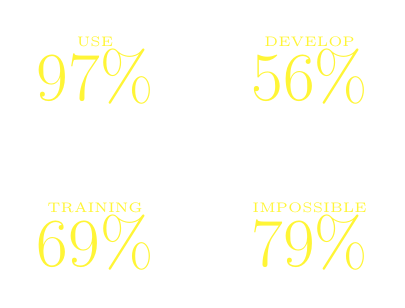
\begin{tikzpicture}
\node [align=center, text=yellow!79] (c1)  {\tiny{USE} \\ \Huge{97\%}};
\node[align=center,text=yellow!79, right=of c1] (c2)
{\tiny{DEVELOP}\\ \Huge{56\%}};
\node[align=center,text=yellow!79, below=of c2] (c3)
{\tiny{IMPOSSIBLE}\\ \Huge{79\%}};
\node[align=center,text=yellow!79   , left=of c3] (c3)
{\tiny{TRAINING}\\ \Huge{69\%}};
\end{tikzpicture}
\end{center}
\end{figure}
\tiny{https://www.software.ac.uk/blog/2016-09-12-its-impossible-conduct-research-without-software-say-7-out-10-uk-researchers}
\end{frame}

\begin{frame}
    \begin{itemize}
        \item Unittests
    \end{itemize}
\end{frame}

\begin{frame}[fragile]
\begin{figure}
\textbf{'main.py'}
\begin{minted}
        [
        framesep=2mm,
        baselinestretch=1,
        bgcolor=DarkGray,
        fontsize=\small,
        ]
        {python}
def absolute_value(x):
    if x < 0:
        return -x
    else:
        return x
\end{minted}
\end{figure}
\pause
\begin{figure}
\textbf{'test\_main.py'}
\begin{minted}
        [
        framesep=2mm,
        baselinestretch=1,
        bgcolor=DarkGray,
        fontsize=\small,
        ]
        {python}
import unittest
import main

class TestExample(unittest.TestCase):

    def test_absolute(self):
        self.assertEqual(main.absolute_value(-2), 2)
        self.assertTrue(main.absolute_value(-2), 2)
        self.assertEqual(main.absolute_value(-3),
                         main.absolute_value(3))
        self.assertTrue(main.absolute_value(-2) >= 0)
\end{minted}
\end{figure}
\end{frame}

\begin{frame}[fragile]
\begin{minted}
        [
        framesep=2mm,
        baselinestretch=1,
        bgcolor=DarkGray,
        fontsize=\small,
        ]
        {python}
python -m unittest test_main.py
\end{minted}
\pause
\begin{minted}
        [
        framesep=2mm,
        baselinestretch=1,
        bgcolor=DarkGray,
        fontsize=\small,
        ]
        {python}
---------------------------------
Ran 1 test in 0.000s

OK
\end{minted}
\end{frame}

\begin{frame}
    \begin{itemize}
        \item Unittests
        \item Doctests
    \end{itemize}
\end{frame}

\begin{frame}[fragile]
\begin{figure}
\textbf{'main.py'}
\begin{minted}
        [
        framesep=2mm,
        baselinestretch=1,
        bgcolor=DarkGray,
        fontsize=\small,
        ]
        {python}
import unittest

def absolute_value(x):
    """
    Return the absolute value of an argument.

    For example:

                >>> absolute_value(-2)
                2
                >>> absolute_value(3)
                3
    """
    if x < 0:
        return -x
    else:
        return x
\end{minted}
\end{figure}
\pause
\begin{minted}
        [
        framesep=2mm,
        baselinestretch=1,
        bgcolor=DarkGray,
        fontsize=\small,
        ]
        {python}
python -m doctest main.py
\end{minted}
\end{frame}

\begin{frame}
	\begin{center}
		\huge{\textbf{}}\\~\\
		\small{@NikoletaGlyn}\\
		\small{https://github.com/Nikoleta-v3}\\
	\end{center}
\end{frame}

\end{document}




